The top production cross-section is substantially higher than the
$\WW$ cross-section.  Thus the background due to top quarks represents
a significant challenge for studies of the $\WW$ final state,
including $H \to \WW$ searches.

As explained in Section~\ref{sec:sel_toptag}, we use a dedicated top
tagging veto, which relies on identifying $b$-quarks from top decay to
further suppress the top background.  By assessing the tagging
efficiency and applying this to the number of tagged events, we can
estimate the residual top background after the veto.  Since details
of the jet fragmentation cannot be reliably simulated at low energy,
the tagging efficiency should be estimated from data.

Due to strong dependence of the tagging efficiency on the jet $\pt$, 
the data control samples should have
similar properties to the signal samples.  Thus the method to extract
the background depends on the jet bin.  Additionally, the $\ttbar$ and
$tW$ processes have different tagging efficiency due to difference in 
the number of taggable $b$-quarks. The uncertainty on the expected ratio 
of the event yields for the two processes represents one of the systematic
uncertainties of the top background estimation.

The methods used are now described for each jet bin.  The background
in the control samples is subtracted using a combination of
data-driven methods and simulated events, using the same techniques
explained in this section. The background fractions are at the level
of a few percent of the total sample.

%
% ZERO JETS
%
\subsubsection{Zero-Jet Bin Method}
We perform the measurement of the tagging efficiency for a $b$-quark 
that leads to a low $p_T$ jet or no jet at all in a top control 
sample with exactly one counted jet, which is dominated by $t \bar t$. 
To increase the purity of the $t\bar{t}$ events in this sample, 
we apply $b$-tagging requirements to
the counted jet. The purity of this control sample, as estimated from
simulation, is 97\%.  

We define $\varepsilon^{soft}_{top-tag}$ as:
$$\varepsilon^{soft}_{top-tag} = \frac{N^{control}_{top-tag}}{N^{control}}$$ 

where $N^{control}$ is the number of events in the top control sample,
and $N^{control}_{btag}$ is the number of events in the top control
samples that are tagged by either soft muon tagging or the low-$p_T$
b-jet tagging looking at the rest of the events outside the counted
jet.  The idea is that for \ttbar\ events reconstructed as 1-jet
events, the counted jet is one of the $b$-quarks, while the other one
does not produce a countable jet and has similar kinematics to the
$b$-quarks in the 0-jet events. The efficiency to tag a top event in
the zero-jet bin is thus
$$\varepsilon_{0-jet} = f_{\ttbar}(1 - (1-\varepsilon^{soft}_{top-tag})^2)+f_{tW}\varepsilon^{soft}_{top-tag}$$

where $f_{\ttbar}$ and $f_{tW}$ are the corresponding fraction of 
$\ttbar$ and $tW$ events, respectively, with $f_{tW} \equiv 1-f_{\ttbar}$. 
An important ingredient is the ratio of $\ttbar$ and 
$tW$ cross-sections, for which we assume an uncertainty of 17\%~\cite{XS}. 
The fraction of $\ttbar$ events in the 0-jet bin sample is 
approximately 75\%, after all $\WW$ requirements except the top veto.

In simulated top events $\varepsilon^{soft}_{top-tag}$ is estimated to be
($35 \pm 1$)\%, which leads to a predicted efficiency in the zero-jet
bin of ($53 \pm 1$)\%. This is consistent with the value obtained in
simulated top events in the zero-jet bin of ($55 \pm 2$)\%.
This represents a closure test of the method on simulation.

\begin{figure}[!htbp]
\begin{center}
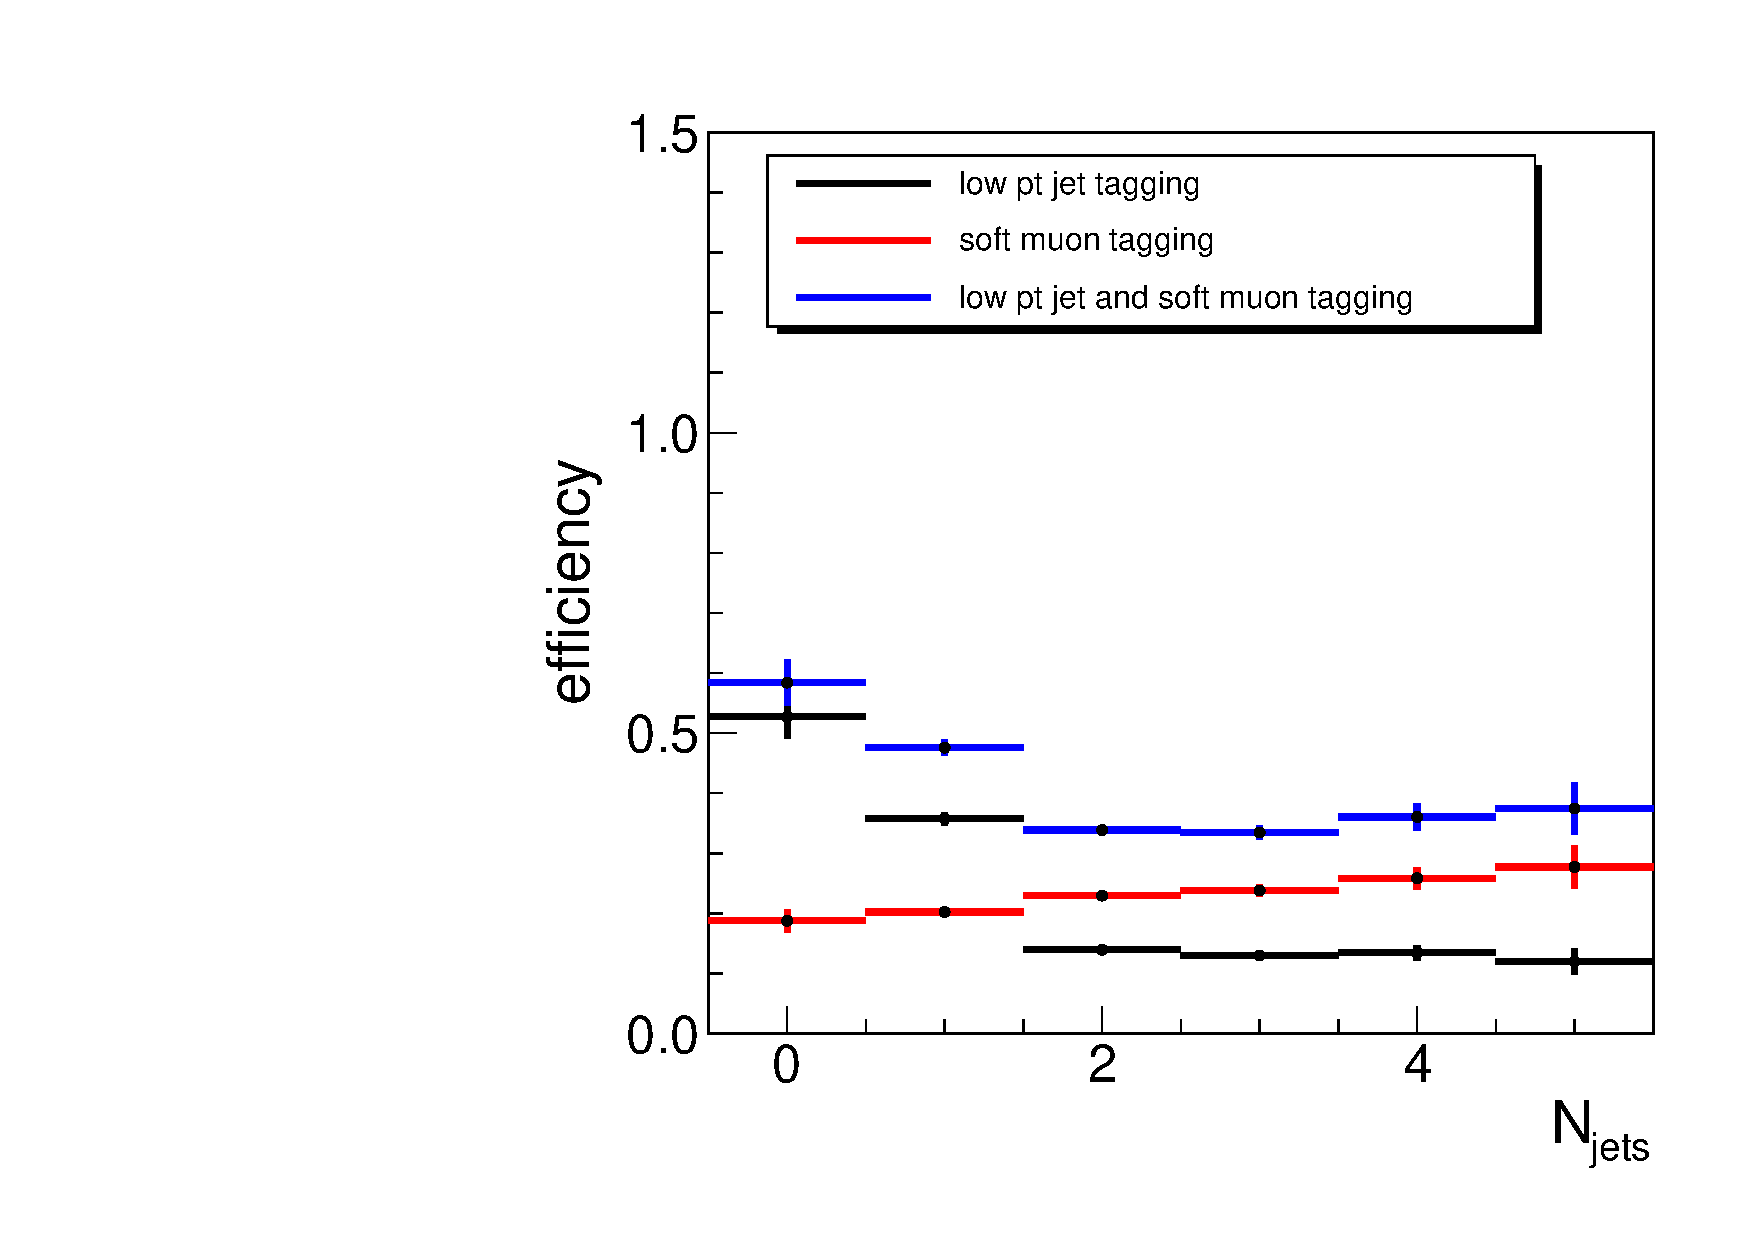
\includegraphics[width=0.60\textwidth]{figures/btag_njets_lowpttagging.pdf}
\caption{Tagging efficiency for low $\pt$ jets, soft muon tagging efficiency 
and the combination of both of them for top simulated events as a function 
of the number of reconstructed jets in top events after applying the 
$\WW$-like selection.}
\label{fig:btag_njets_lowpttagging}
\end{center}
\end{figure}

%
% ONE JET BIN
%
\subsubsection{1-Jet Bin Method}
To measure the tagging efficiency in the 1-jet bin we use top events 
with two reconstructed jets as the control sample. 
The expected tagging efficiency in simulated $t\bar{t}$ events after the $WW$ preselection
is shown using all jets and soft-muons and for the highest $\pt$ jet only
as a function of the number of counted jets in Figure~\ref{fig:btag_njets_highestptjet}.
The tagging efficiency for the highest $\pt$ jet is approximately
the same for the 1-jet and 2-jet bins. Therefore, we use the 
tagging on the highest $\pt$ jet and measure its efficiency in
the 2-jet bin where, in order to increase the top purity, 
the second jet is required to be b-tagged.

\begin{figure}[!htbp]
\begin{center}
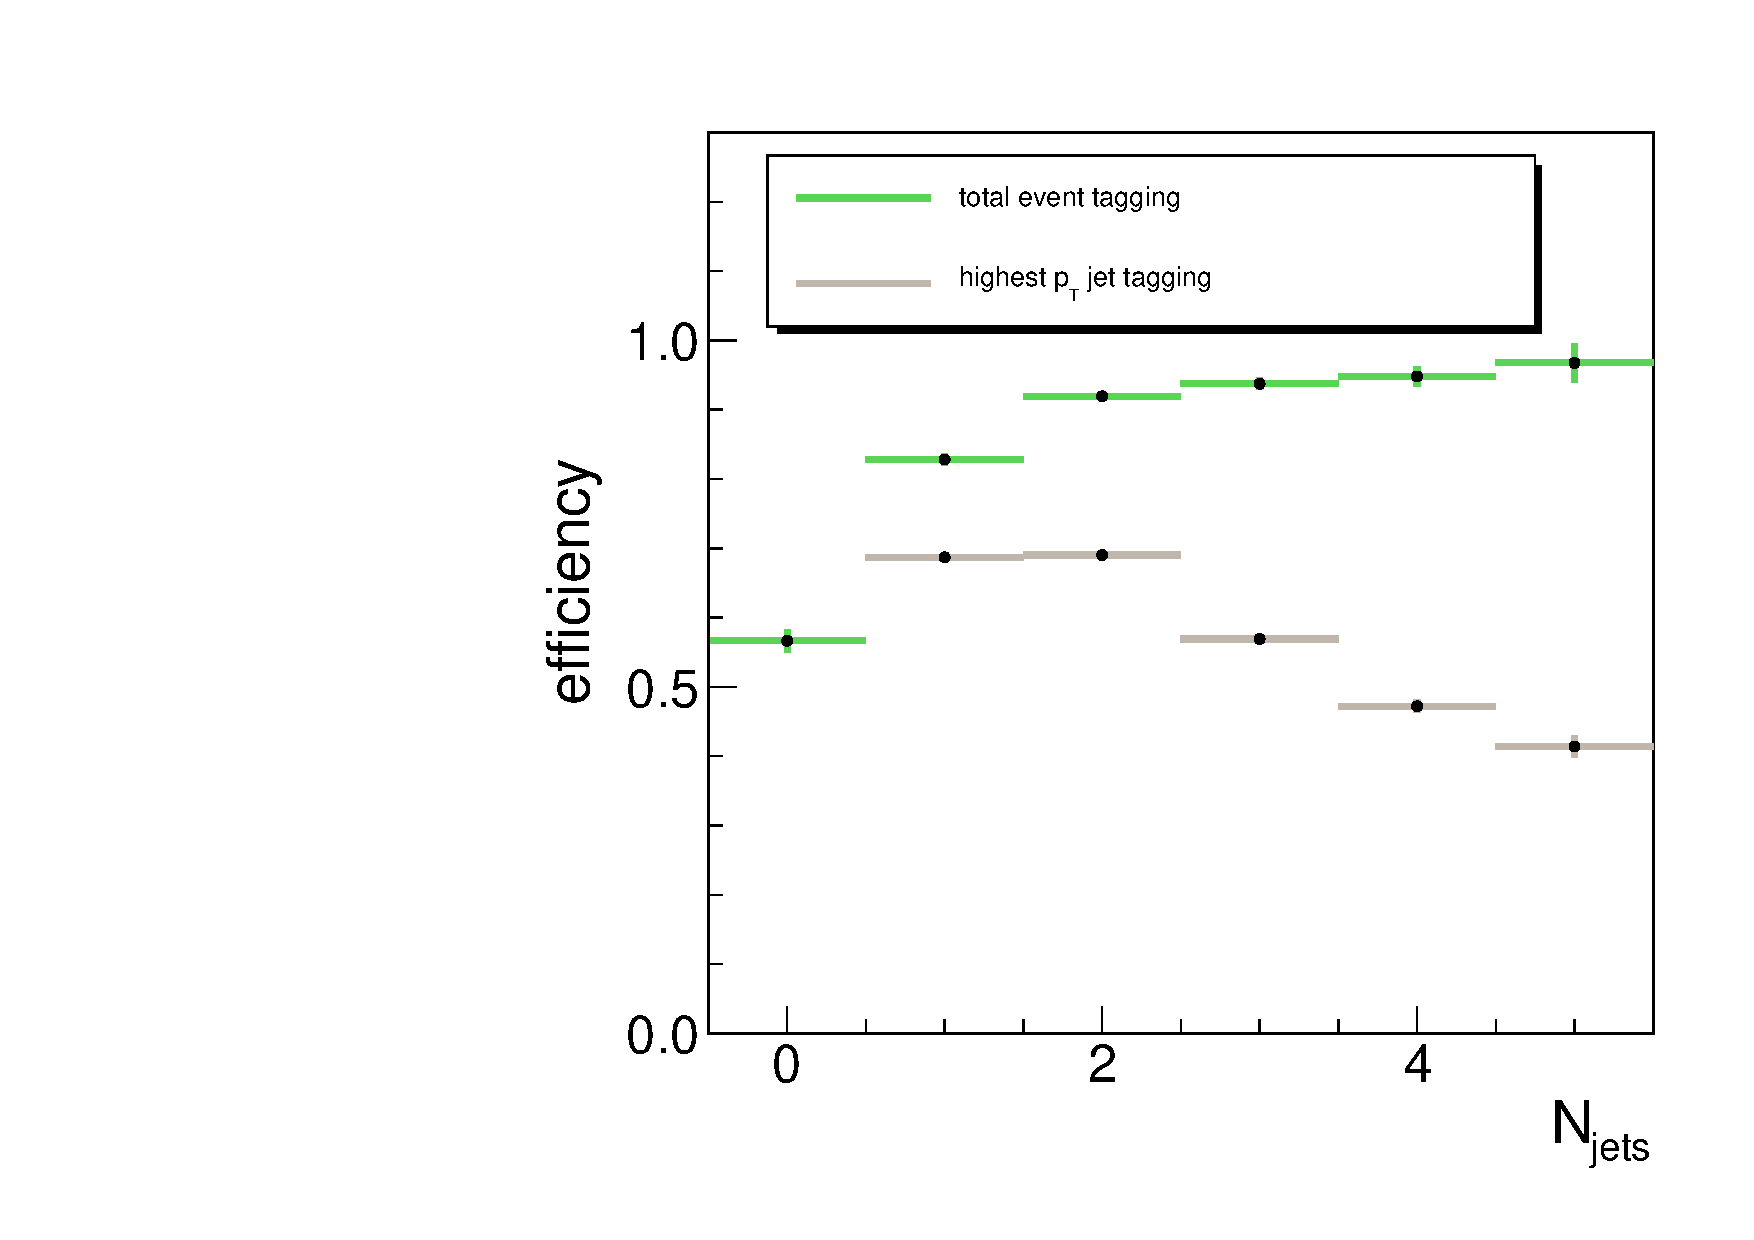
\includegraphics[width=0.55\textwidth]{figures/btag_njets_highestptjet.pdf}
\caption{Total tagging efficiency and tagging efficiency for the highest
$\pt$ jet for simulated top events as a function of the number of reconstructed
jets in top events after applying the $\WW$-like selection.}
\label{fig:btag_njets_highestptjet}
\end{center}
\end{figure}

The residual number of top events in the 1-jet bin is then given by,
$${N_{no~tagged}^{1-jet} = N_{tagged}^{1-jet} \times (1-\epsilon_{highest~\pt~jet})/\epsilon_{highest~\pt~jet}},$$
where $N_{tagged}^{1-jet}$ is the number of events where the counted jet is
tagged and none of the other non-counted jets are tagged, and $\epsilon_{highest~\pt~jet}$ is the 
tagging efficiency for the highest $p_{T}$ jet measured from the 2-jet bin.
The closure test, comparing the estimate using this procedure with 
the simulation, gives agreement to within $1\%$.

%
% VBF
% 
\subsubsection{2-Jet Bin Method}
Estimation of the top background in the 2-jet bin is complicated due to 
the additional requirements applied to the jets to
select $qqH$-like events. The tagging effiency for the selected jets 
after applying such selection is smaller than that in the inclusive 
2-jet bin sample, since the selection enhances events with forward 
jets, which have lower tagging efficiency.

The proposed method is to measure the tagging efficiency of the most central 
jet in the event as a function of its $\pt$ and $\eta$ in an inclusive top 
enriched control sample, and then apply that rate to fully selected events 
where the most central jet is top tagged. In this way the 
possible kinematical differences between the control and signal regions 
are taken into account.

Therefore, the residual number of top events in the 2-jet bin after applying the full 
$qqH$-like is given by,
$${N_{non~tagged}^{qqH} = N_{tagged}^{qqH} \times (1-\epsilon_{central~jet})/\epsilon_{central~jet}},$$
where $N_{no~tagged/tagged}^{qqH}$ is the number non-tagged/tagged events using 
the most central jet, and $\epsilon_{central~jet}$ is the 
tagging efficiency as a function of $\pt$ and $\eta$ of the jet. The comparison of the 
$|\eta|$ distribution of the most central jet in top events after applying the $qqH$-like selection between the simulation and 
the prediction using top-tagged events is shown in Figure~\ref{fig:vbf_btagprediction_jetmin}, where 
good agreement in shape and normalization is observed in the region $|\eta|<2.5$. A small correction 
of about 10\% in the yield must be included in the prediction to take into account the fraction 
of top events where the most central jet is outside the tracker acceptance.

\begin{figure}[!htbp]
\begin{center}
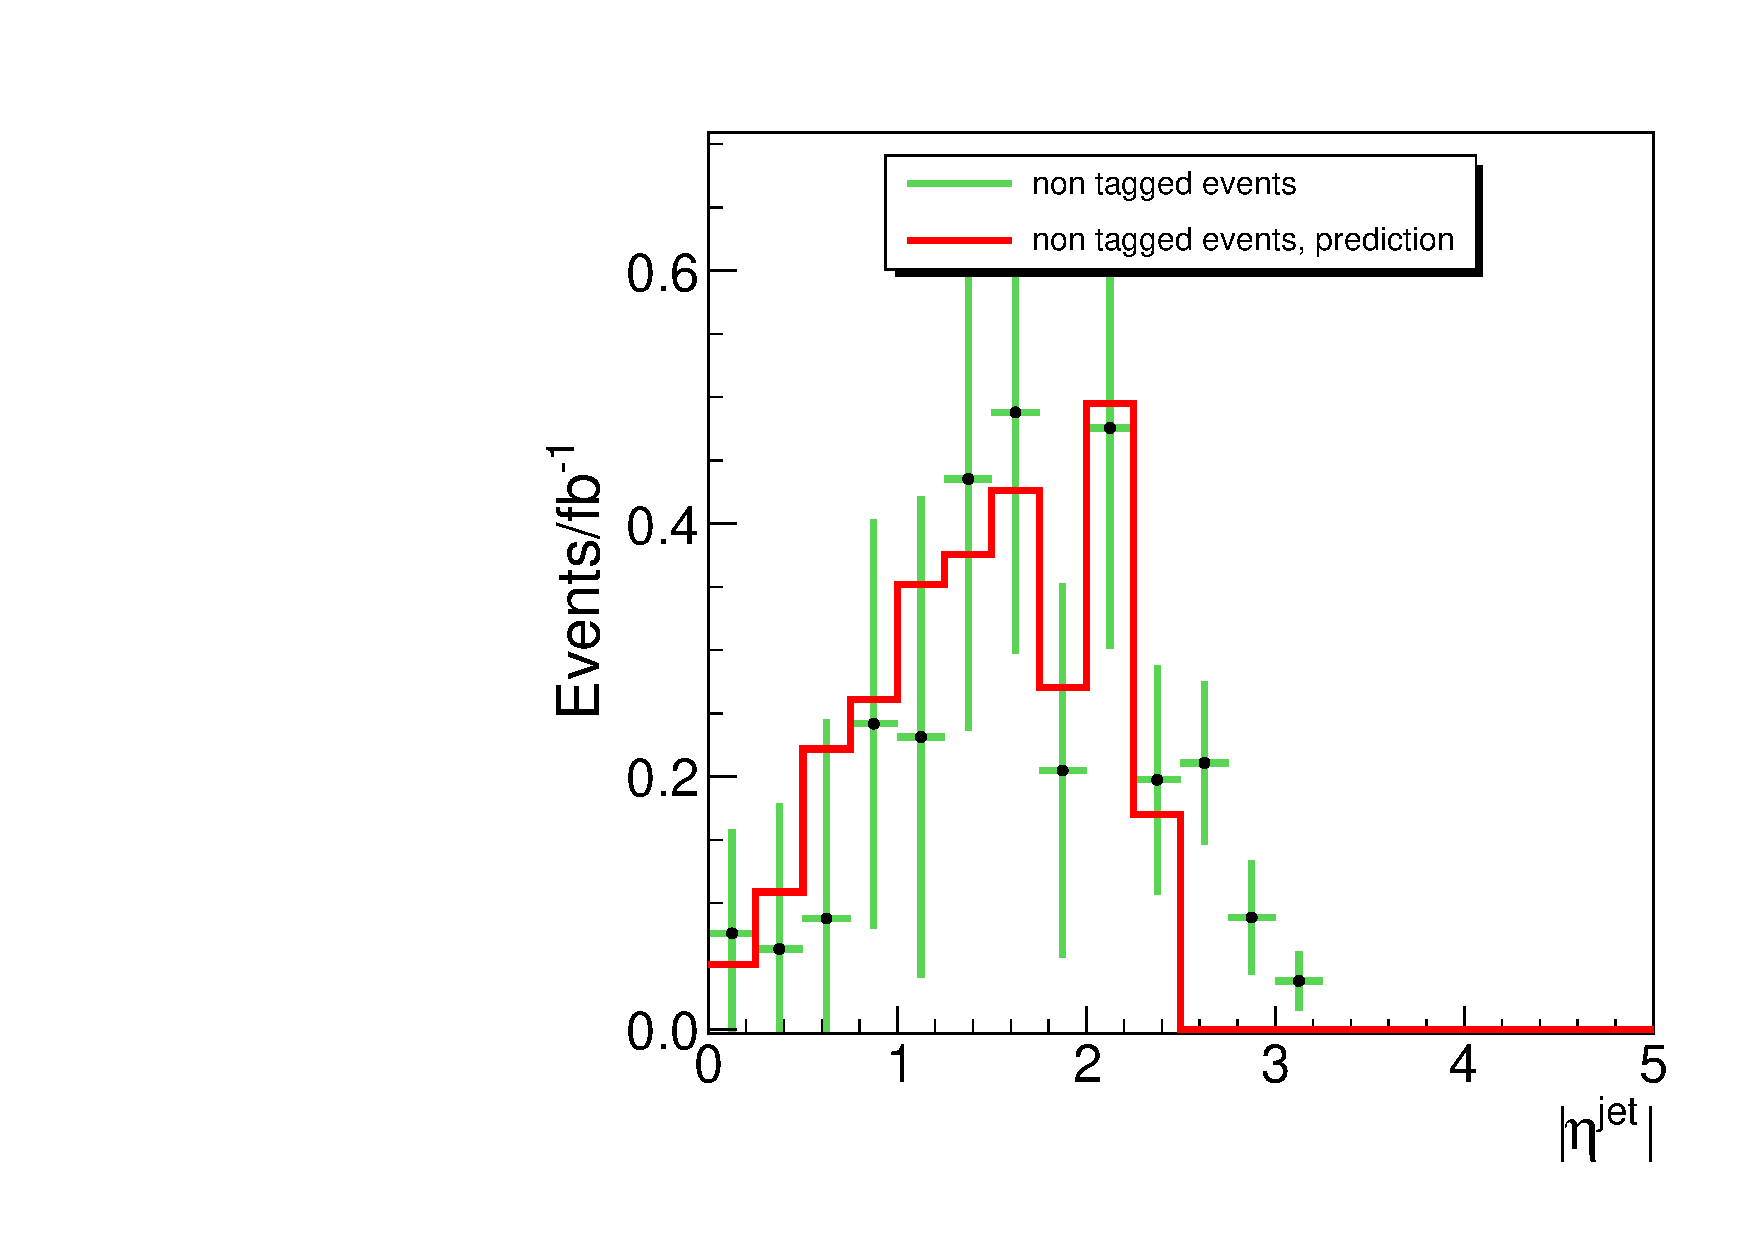
\includegraphics[width=0.65\textwidth]{figures/vbf_btagprediction_jetmin.pdf}
\caption{$|\eta|$ distribution of the most central jet in top events after 
applying the $qqH$-like selection. Comparison between the simulation and 
the prediction using top-tagged events.}
\label{fig:vbf_btagprediction_jetmin}
\end{center}
\end{figure}

The extrapolation from the $b$-tag region is performed by means of a bayesian model, built with 
JAGS~\cite{jags}, that relies on the knowledge of the $\eta$ shape of the $b$-vetoed jet (signal region) 
for the ttbar sample from MC. Assuming the statistics in this region to be multinomial, 
and by using the $b$-tagging efficiency measured from data, the model is built, 
to be used to extrapolate a measurement in the $b$-tag region to the signal region. 
For $\intlumi$, from the measured distribution of 5 $b$-tag events in the control region, 
distributed in $\eta$ according to the simulation expectations, 
the extrapolated number of events in the signal region is $3.4\pm 2.3$,
to be compared to the expectation of 2.83. 
The uncertainty on the estimate is evaluated as the RMS of the distribution in the signal region, 
around its peak. Therefore, it accounts both for the statistics fluctuations and for the systematics of 
the technique.
Assuming the statistics fluctuations to be poissonian, the remaining systematic part is of the order of 40\%. 

%jets and soft muons in the event, which has little correlation 
%with the two tagging jets. The tagging efficiency for the combination of 
%low $\pt$ jets and soft muons after and before applying the $qqH$-like 
%selection, and after and before requiring that the two highest $\pt$ jets 
%in the event are not tagged is shown in 
%Figure~\ref{fig:btag_njets_vbfcuts}. We see that just by requiring the two 
%highest $\pt$ jets in the event not tagged, the agreement in the 2-jet 
%bin is rather good.

%The proposed method is to measure the tagging efficiency using low $\pt$ 
%jets and soft muons in the event, which has little correlation 
%with the two tagging jets. The tagging efficiency for the combination of 
%low $\pt$ jets and soft muons after and before applying the $qqH$-like 
%selection, and after and before requiring that the two highest $\pt$ jets 
%in the event are not tagged is shown in 
%Figure~\ref{fig:btag_njets_vbfcuts}. We see that just by requiring the two 
%highest $\pt$ jets in the event not tagged, the agreement in the 2-jet 
%bin is rather good.

%\begin{figure}[!htbp]
%\begin{center}
%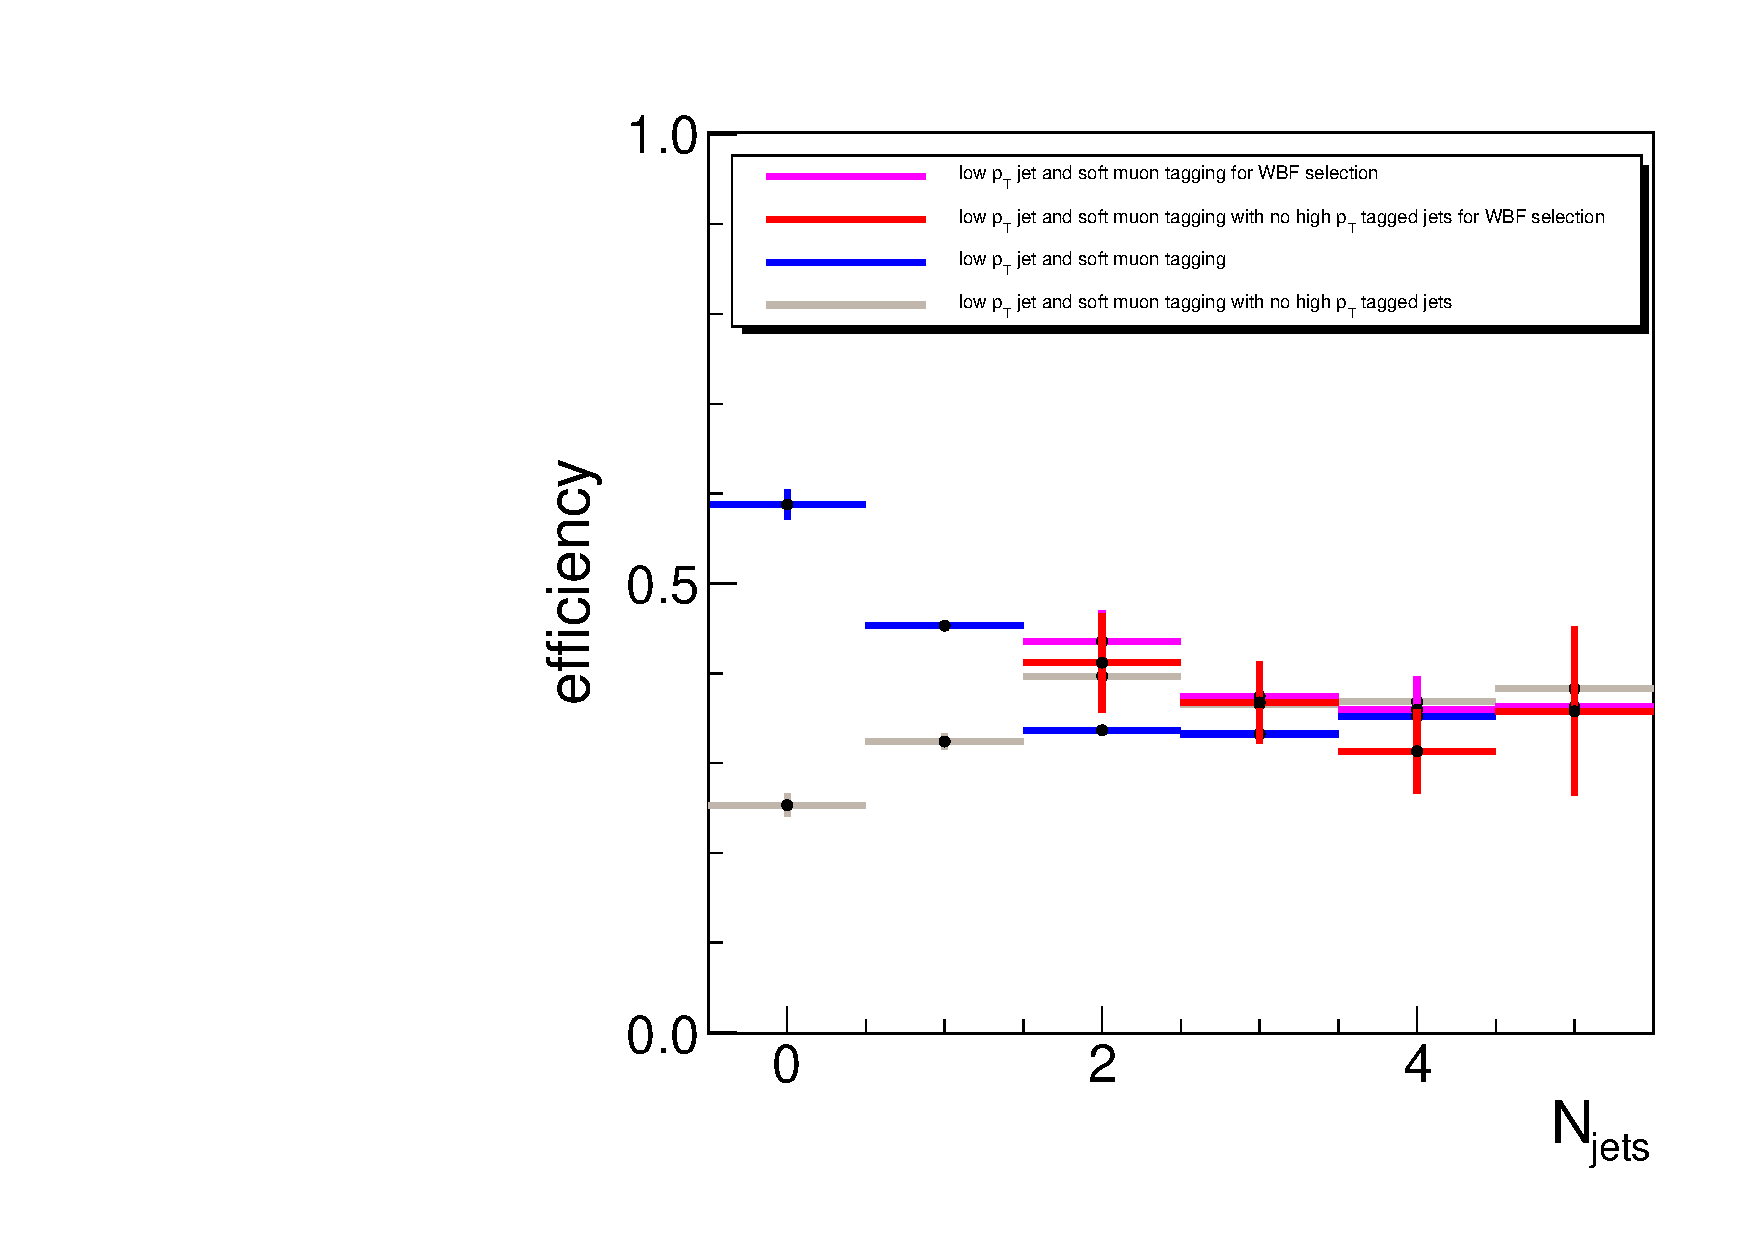
\includegraphics[width=0.65\textwidth]{figures/btag_njets_vbfcuts.pdf}
%\caption{Tagging efficiency for the combination of 
%low $\pt$ jets and soft muons after and before applying the $qqH$-like 
%selection, and after and before requiring that the two highest $\pt$ jets 
%in the event are not tagged.}
%\label{fig:btag_njets_vbfcuts}
%\end{center}
%\end{figure}

%Therefore, the residual number of top events in the 2-jet bin after applying the full 
%$qqH$-like is given by,
%$${N_{no~tagged}^{qqH} = N_{tagged}^{qqH} \times (1-\epsilon_{soft~jets})/\epsilon_{soft~jets}},$$
%where $N_{no~tagged/tagged}^{qqH}$ is the number of events where the event is no-tagged/tagged by either low $\pt$ 
%jets or soft muons, and $\epsilon_{soft~jets}$ is the 
%tagging efficiency for low $\pt$ jets and soft muons measured from the 2-jet bin for events where the two 
%highest $\pt$ jets in the event not $b$-tagged. The closure test, comparing the estimate using 
%this procedure with the simulation, gives agreement to within $5\%$.

\subsubsection{Results on data}
The MC prediction for the top background after the $WW$ preselection 
is compared with the observed event counts in the data-driven estimation
in Table~\ref{tab:ttbar_est1}. The analyzed data correspond to \intlumi.

\begin{table}
\begin{center}
\begin{tabular}{l c c c}
\hline
Sample                                        &   0-jet           & 1-jet           \\
\hline
Estimated top events in simulation  	      &   36.6 $\pm$ 1.6  & 112.0 $\pm$ 6.1 \\
tagging efficiency (\%)                       &    52  $\pm$  8   &  66  $\pm$ 2    \\
top-tagged events in data           	      &          92       &    305          \\
background events in control region           &    23.3  $\pm$ 4.6&   13.5 $\pm$ 3.7\\
Data-driven top background estimate           &  63.7 $\pm$ 15.9  & 144.5 $\pm$ 15.1\\
\hline
\end{tabular}
\end{center}
\caption{Predictions of the top background contribution compared 
with observed event counts in the data-driven estimation (first method)
after the $WW$ preselection. 
The analyzed data correspond to \intlumi.
The uncertainties are 
statistical only. The systematic uncertainties are expected to be 
negligible at this level or precision.\label{tab:ttbar_est1}}
\end{table}

The extrapolation from the $\WW$ region to each $H \to \WW$ region is obtained from simulated events. 

%\subsubsection{Data Results}
%This section describes the tagging efficiency results obtained in data, 
%and the comparison of the residual background predictions obtained from
%the methods described above with simulation expectations.

%The tagging efficiency for the combination of low $\pt$ jets 
%and soft muons as a function of the number of counted jets on data and 
%simulation is shown in Figure~\ref{fig:btag_njets_lowpttagging_data}. 
%The total tagging efficiency as a function of the number of reconstructed jets on data 
%and simulation is shown in Figure~\ref{fig:btag_njets_totaltagging_data}. 
%The tagging efficiency for the leading jet $\pt$ as a function of the number of 
%reconstructed jets on data and simulation is shown in 
%Figure~\ref{fig:btag_njets_highestptjet_data}. 
%In all cases a reasonable agreement is found between the data 
%and the simulation, although the statistical uncertainty is large.

%\begin{figure}[!htbp]
%\begin{center}
%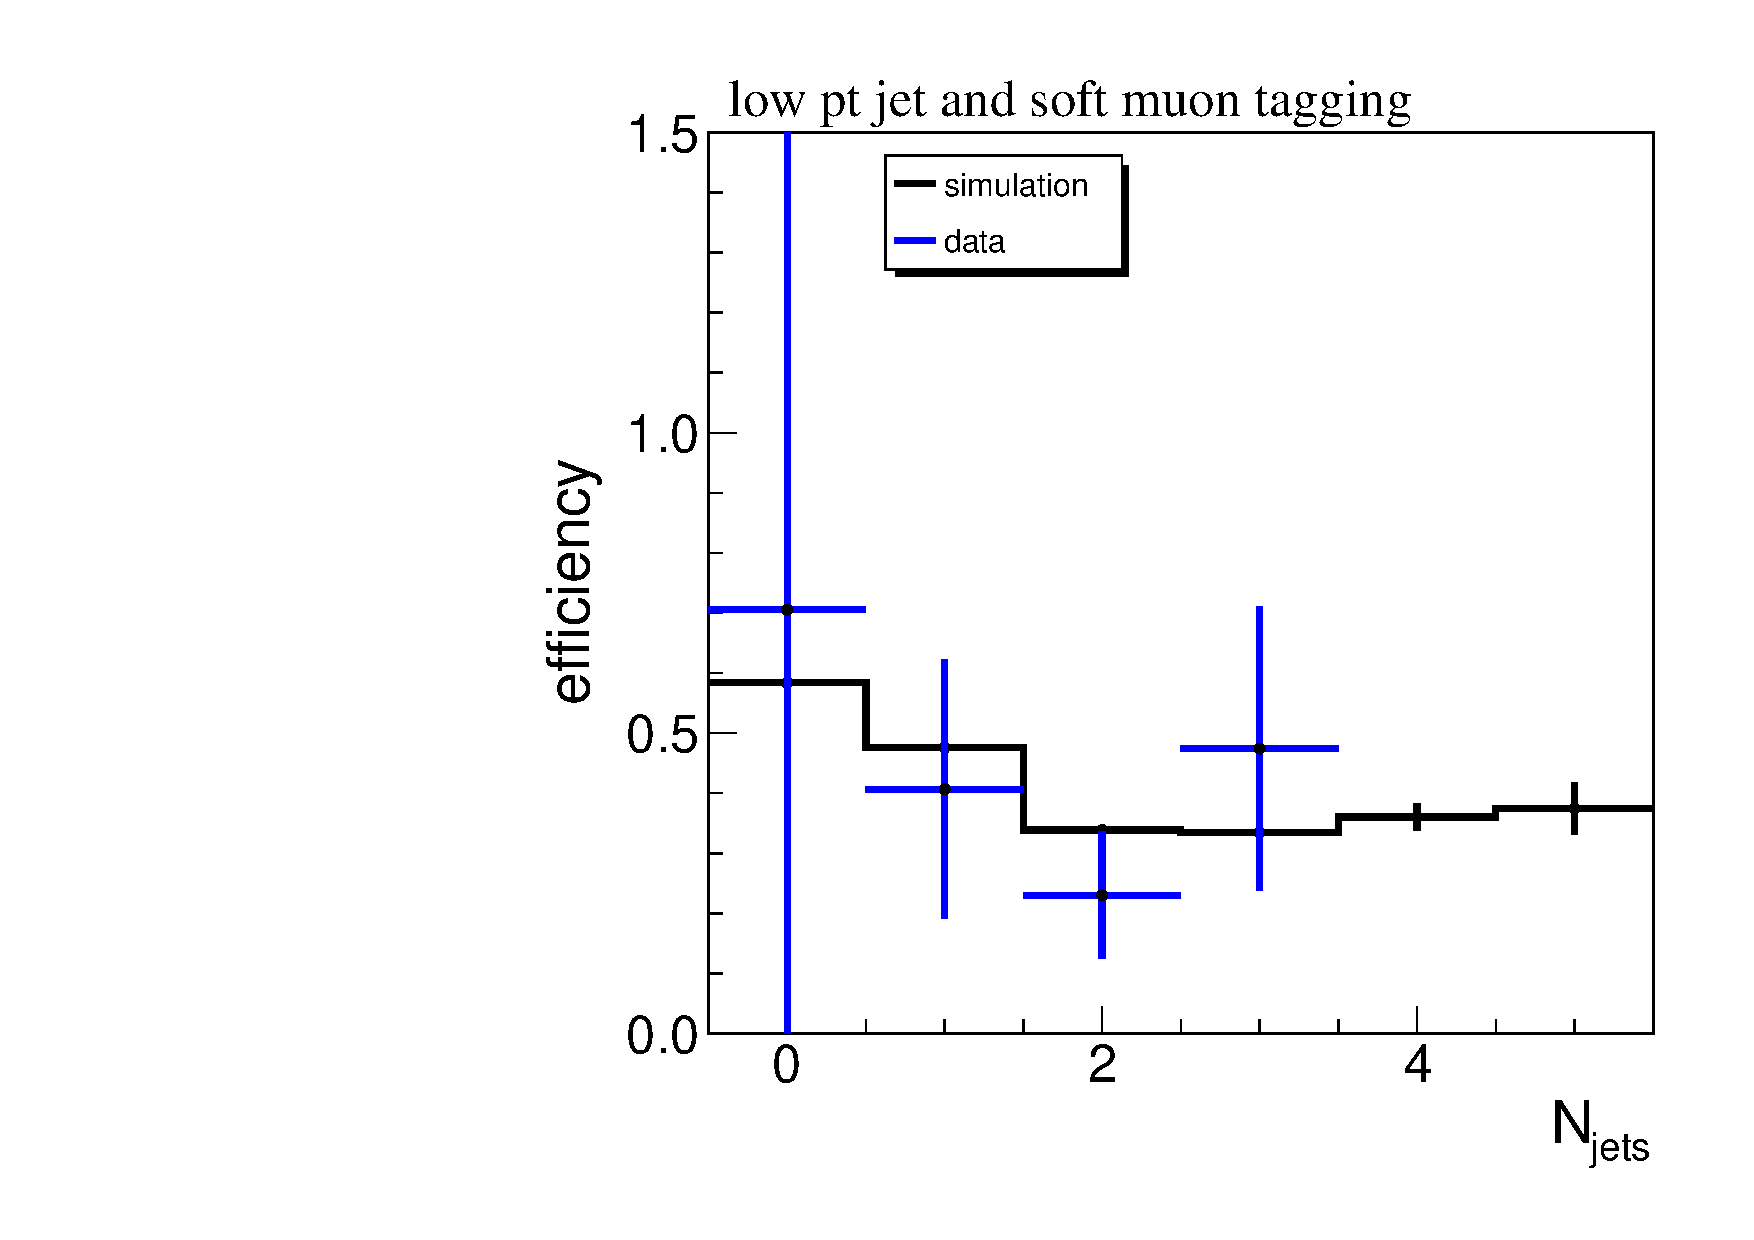
\includegraphics[width=0.55\textwidth]{figures/btag_njets_lowpttagging_data.pdf}
%\caption{Tagging efficiency for the combination of low $\pt$ jets and soft muons 
%as a function of the number of counted jets after applying 
%the $\WW$-like selection on data and simulation.}
%\label{fig:btag_njets_lowpttagging_data}
%\end{center}
%\end{figure}

%\begin{figure}[!htbp]
%\begin{center}
%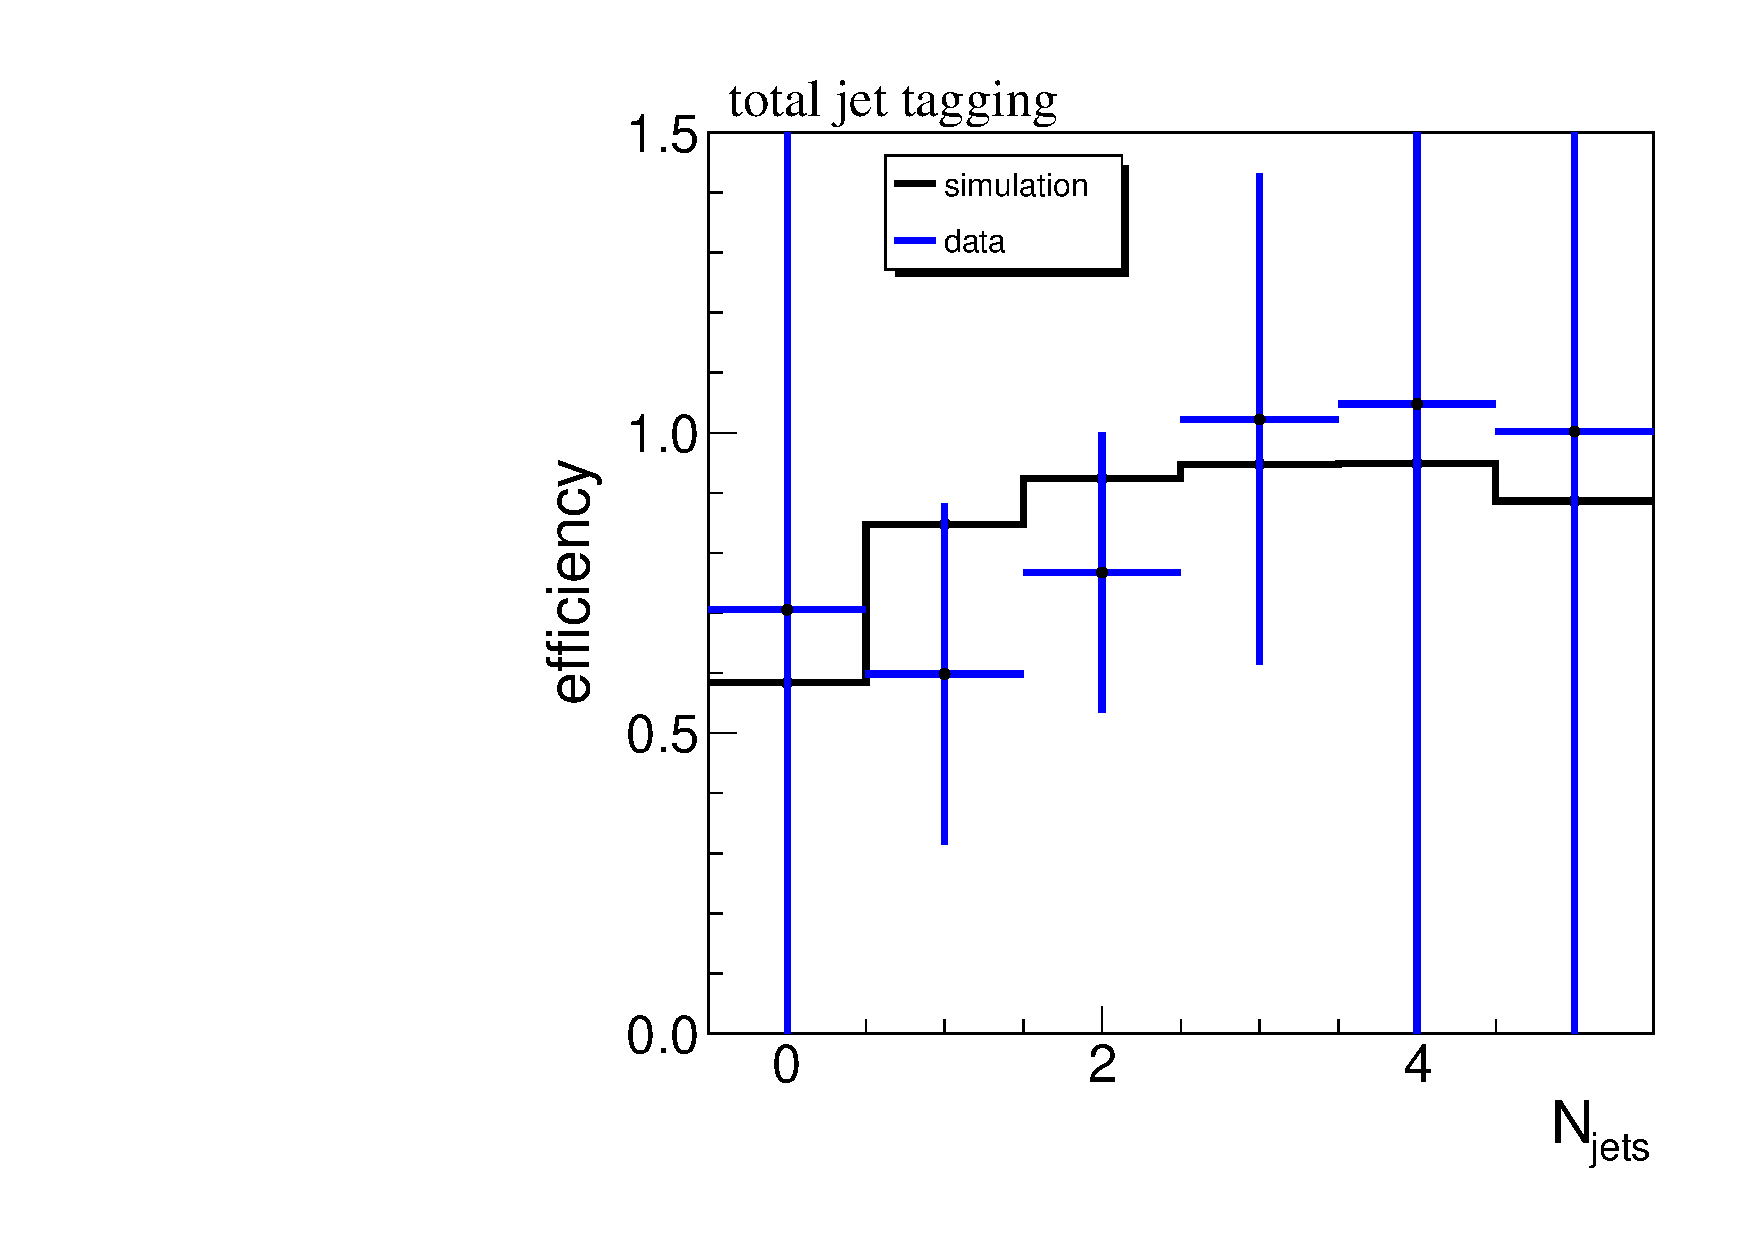
\includegraphics[width=0.55\textwidth]{figures/btag_njets_totaltagging_data.pdf}
%\caption{The total tagging efficiency as a function of the number of counted 
%jets after applying the $\WW$-like selection on data and simulation.}
%\label{fig:btag_njets_totaltagging_data}
%\end{center}
%\end{figure}

%\begin{figure}[!htbp]
%\begin{center}
%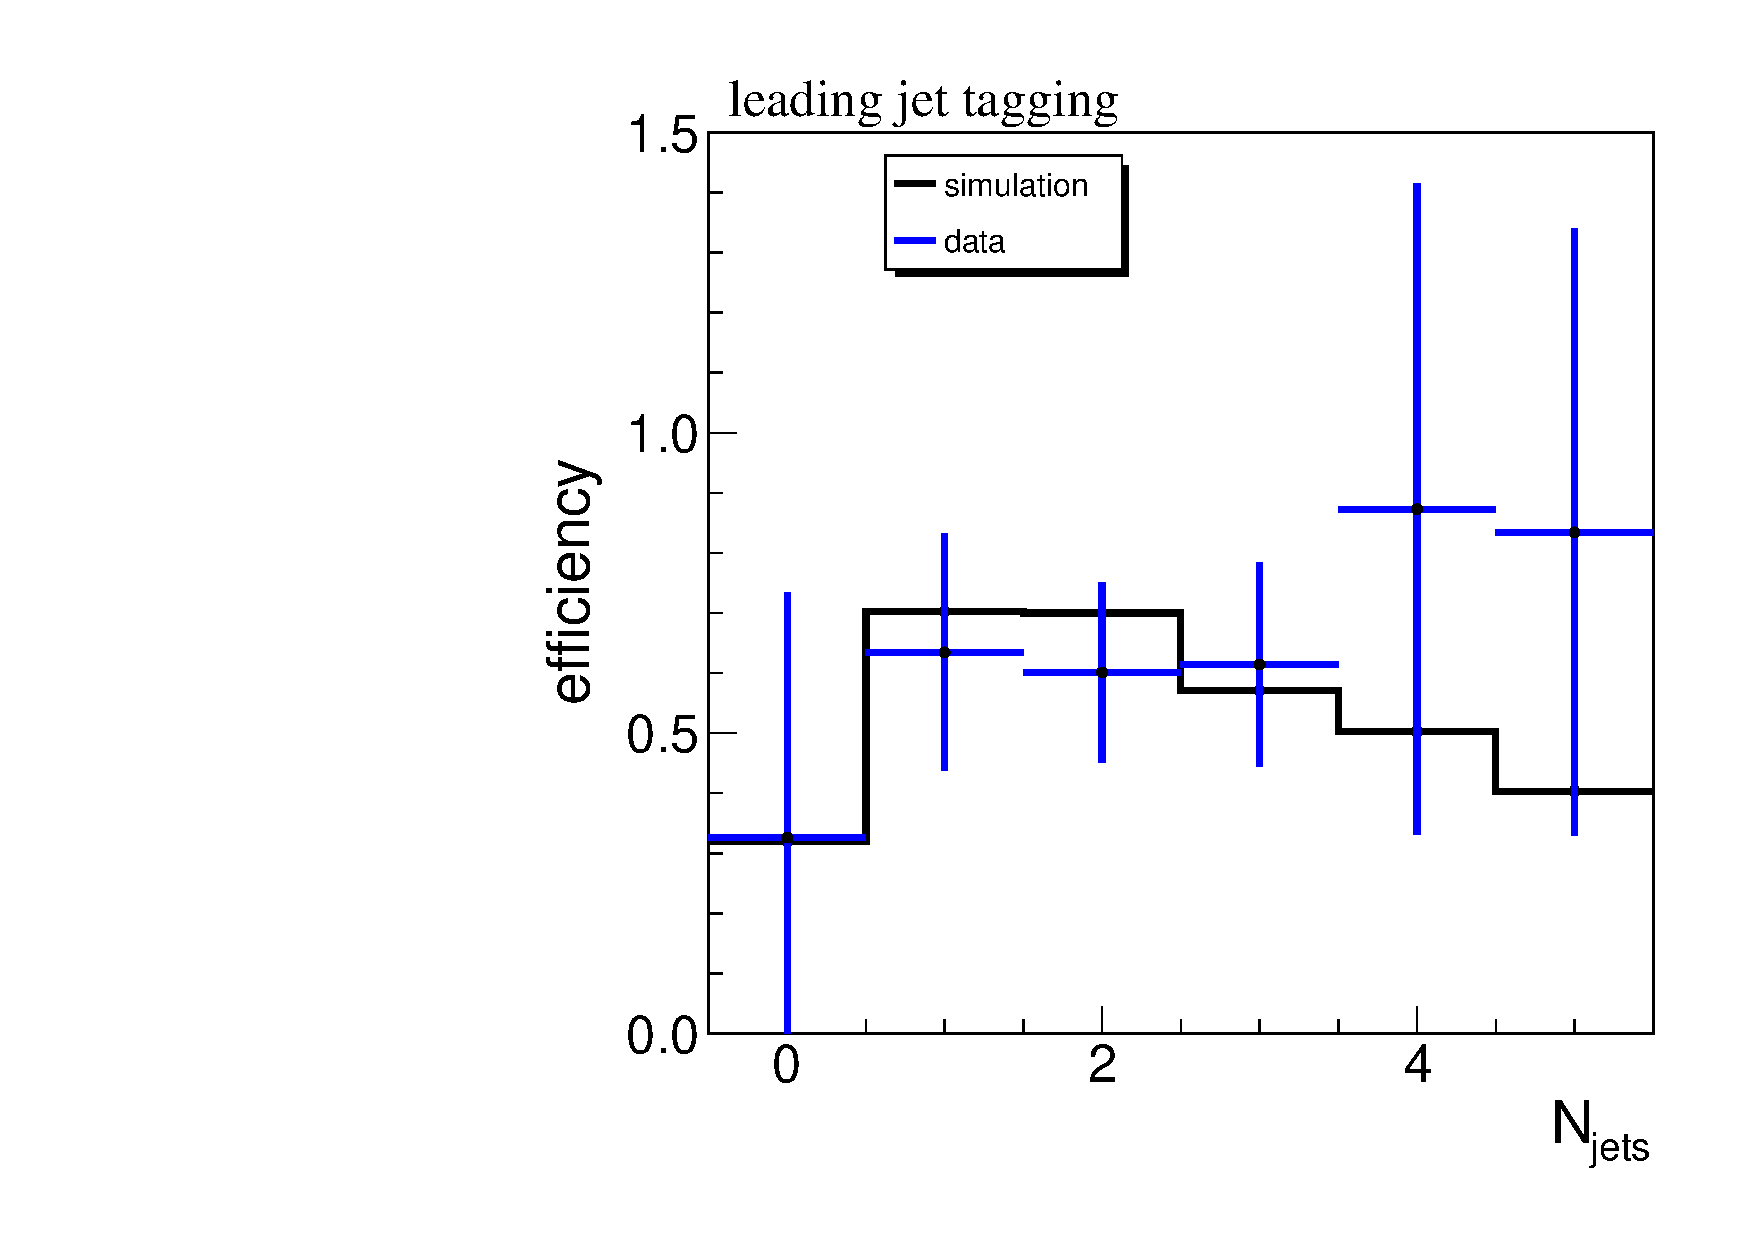
\includegraphics[width=0.55\textwidth]{figures/btag_njets_highestptjet_data.pdf}
%\caption{Tagging efficiency for the leading jet $\pt$ as a function of the number of counted 
%jets after applying the $\WW$-like selection on data and simulation.}
%\label{fig:btag_njets_highestptjet_data}
%\end{center}
%\end{figure}
